%Graad 10 Wiskunde Teachers Guide

\newgeometry{paper=a4paper, lmargin=0.1\paperwidth, rmargin=0.1\paperwidth, tmargin=1in, bmargin=1in}

\begin{titlepage}
    \thispagestyle{empty}
    \vspace*{1in}
    {\centering\normalfont\sffamily\fontsize{36}\normalfont\itshape{Everything Maths\\}\vspace*{1cm}}
    {\centering\normalfont\sffamily\fontsize{22}\normalfont\itshape{~~Graad 10 Wiskunde -- Onderwysersgids}}
    \vspace*{1in} \\
    {\centering\LARGE 'n Inleiding tot Everything Maths vir Graad 10 \\
   {\vspace*{1in}
     deur Siyavula en vrywilligers \\}

\begin{center}

\includegraphics[width=0.4\textwidth]{siyavulasmall.png}
\end{center}
\vfill
\begin{center}
\begin{minipage}{0.4\textwidth}

\includegraphics[width=0.7\textwidth]{dbelogo.png}
\end{minipage}
\hspace*{1.0cm}
\begin{minipage}{0.40\textwidth}

\includegraphics[width=1.1\textwidth]{shuttleworthfunded.png}
\end{minipage}
\end{center}

\end{titlepage}


\newpage
\thispagestyle{empty}
\mbox{}

\newpage
\begin{center}
    \thispagestyle{empty}

    \vspace*{4in}

    {\normalfont\sffamily\fontsize{36}\normalfont\itshape{Everything Maths } \\ \vspace*{1cm}
    {\normalfont\sffamily\fontsize{22}\normalfont\itshape{Grade 10 Wiskunde}}
    \vspace*{1in} \\
    \LARGE Weergawe 1 -- CAPS \\

   {\vspace*{2in}
     deur Siyavula en vrywilligers \\

ISBN: 978-1-920423-11-7
  

\vfill

    }}

\end{center}






% Copyright notice
\newpage
\thispagestyle{empty}
{
\begin{center}
\normalfont\sffamily\fontsize{22}\normalfont\itshape Kopiereg kennisgewing\\

\vspace*{1in}

\textbf{Jou wetlike vryheid om hierdie boek te kopieer}\\

\end{center}
}

{\LARGE
Jy mag enige gedeelte van hierdie boek vrylik kopieer, trouens ons moedig jou aan om dit doen. Jy kan dit soveel keer as jy wil fotostateer, uitdruk of versprei. Jy kan dit op jou selfoon, iPad, rekenaar of geheue stokkie aflaai. Jy kan dit selfs op ‘n kompakskyf (CD) brand of dit vir iemand per e-pos aanstuur of op jou eie webblad laai.
Die enigste voorbehoud is dat jy die boek, sy omslag en die kortkodes onveranderd laat. \par

Vir meer inligting oor die Creative Commons Attribution-NoDerivs 3.0 Unported (CC BY-ND
3.0) lisensie besoek \underline{http://creativecommons.org/licenses/by-nd/3.0/}}\par

\vspace*{1in}
\begin{center}
\normalfont\sffamily\fontsize{22}\normalfont\itshape

\textbf{Lys van skrywers}\\

\vspace*{0.7in}

\textbf{Siyavula kernspan}\\
\vspace*{0.05in}
\LARGE Bridget Nash, Alison Jenkin, Marina van Zyl, Nicola du Toit, Heather Williams, Carl Scheffler

\end{center}
}
\vspace*{2in}

\begin{center}
\begin{minipage}{0.6\textwidth}

\includegraphics[width=0.8\textwidth]{../title_images/cc2.png}
\end{minipage}
\begin{minipage}{0.3\textwidth}

\includegraphics[width=0.8\textwidth]{../title_images/cc1.png}
\end{minipage}
\end{center}
}
% % Authors
% \newpage
% \thispagestyle{empty}
% 
% 
% \begin{flushleft} \textbf{\huge Authors List} \end{flushleft}
% 
% {\LARGE This book is based upon the original Free High School Science Text which was entirely written by
% volunteer academics, educators and industry professionals. Their vision was to see a curriculum aligned
% set of mathematics and physical science textbooks which are freely available to anybody and exist
% under an open copyright license.} \par
% 
% \textbf{\LARGE Siyavula core team} \\
% 
% Neels van der Westhuizen; Alison Jenkin; Marina van Zyl; Helen Robertson; Carl Scheffler; Nicola du Toit; Gumani Mudau; Thomas Masango \par
% 
% \textbf{\LARGE Original Free High School Science Texts core team}\\
% 
% Mark Horner; Samuel Halliday; Sarah Blyth; Rory Adams; Spencer Wheaton \par 
% 
% 
% \textbf{\LARGE Original Free High School Science Texts editors}\\
% 
% Jaynie Padayachee; Joanne Boulle; Diana Mulcahy; Annette Nell; René Toerien; Donovan Whitfield \par
% 
% \textbf{\LARGE Siyavula and Free High School Science Texts contributors}\\
% 
%     Sarah Abel;
% Dr. Rory Adams;
%     Andrea Africa;
%     Matthew Amundsen;
%     Ben Anhalt;
%     Prashant Arora;
%     Amos Baloyi;
%     Bongani Baloyi;
%     Raymond Barbour;
%     Caro-Joy Barendse;
%     Richard Baxter;
%     Tara Beckerling;
% Dr. Sarah Blyth;
%     Sebastian Bodenstein;
%     Martin Bongers;
%     Gareth Boxall;
%     Stephan Brandt;
%     Hannes Breytenbach;
%     Alex Briell;
%     Wilbur Britz;
%     Graeme Broster;
%     Craig Brown;
%     Richard Burge;
%     Bianca Böhmer;
%     George Calder-Potts;
%     Eleanor Cameron;
%     Richard Case;
%     Sithembile Cele;
%     Alice Chang;
%     Richard Cheng;
%     Fanny Cherblanc;
% Dr. Christine Chung;
%     Brett Cocks;
%     Stefaan Conradie;
%     Rocco Coppejans;
%     Tim Craib;
%     Andrew Craig;
%     Tim Crombie;
%     Dan Crytser;
% Dr. Anne Dabrowski;
%     Laura Daniels;
%     Gareth Davies;
%     Jennifer de Beyer;
%     Jennifer de Beyer;
%     Deanne de Bude;
%     Mia de Vos;
%     Sean Dobbs;
%     Buhle Donga;
%     William Donkin;
%     Esmi Dreyer;
%     Nicola du Toit;
%     Matthew Duddy;
%     Fernando Durrell;
% Dr. Dan Dwyer;
%     Alex Ellis;
%     Tom Ellis;
%     Andrew Fisher;
%     Giovanni Franzoni;
%     Nina Gitau Muchunu;
%     Lindsay Glesener;
%     Kevin Godby;
% Dr. Vanessa Godfrey;
%     Terence Goldberg;
% Dr. Johan Gonzalez;
%     Saaligha Gool;
%     Hemant Gopal;
% Dr. Stephanie Gould;
%     Umeshree Govender;
%     Heather Gray;
%     Lynn Greeff;
%     Carine Grobbelaar;
% Dr. Tom Gutierrez;
%     Brooke Haag;
%     Kate Hadley;
%     Alex Hall;
% Dr. Sam Halliday;
%     Asheena Hanuman;
% Dr. Nicholas Harrison;
%     Neil Hart;
%     Nicholas Hatcher;
%     Jason Hayden;
%     Laura Hayward;
%     Cho Hee Shrader;
% Dr. Fritha Hennessy;
%     Shaun Hewitson;
%     Millie Hilgart;
%     Grant Hillebrand;
%     Nick Hobbs;
%     Chris Holdsworth;
% Dr. Benne Holwerda;
% Dr. Mark Horner;
%     Robert Hovden;
%     Mfandaidza Hove;
%     Jennifer Hsieh;
%     Laura Huss;
% Dr. Matina J. Rassias;
%     Rowan Jelley;
%     Grant Jelley;
%     Clare Johnson;
%     Luke Jordan;
%     Tana Joseph;
% Dr. Fabian Jutz;
%     Brian Kamanzi;
% Dr. Lutz Kampmann;
%     Simon Katende;
%     Natalia Kavalenia;
%     Nothando Khumalo;
%     Paul Kim;
% Dr. Jennifer Klay;
%     Lara Kruger;
%     Sihle Kubheka;
%     Andrew Kubik;
% Dr. Jannie Leach;
%     Nkoana Lebaka;
% Dr. Tom Leinster;
%     Henry Liu;
%     Christopher Loetscher;
%     Mike Loseby;
%     Amandla Mabona;
%     Malothe Mabutho;
%     Stuart Macdonald;
% Dr. Anton Machacek;
%     Tshepo Madisha;
%     Batsirai Magunje;
% Dr. Komal Maheshwari;
%     Michael Malahe;
%     Masoabi Malunga;
%     Masilo Mapaila;
%     Bryony Martin;
%     Nicole Masureik;
%     John Mathew;
% Dr. Will Matthews;
%     Chiedza Matuso;
%     JoEllen McBride;
%     Dr Melanie Dymond Harper;
%     Nikolai Meures;
%     Riana Meyer;
%     Filippo Miatto;
%     Jenny Miller;
%     Abdul Mirza;
%     Mapholo Modise;
%     Carla Moerdyk;
%     Tshwarelo Mohlala;
%     Relebohile Molaoa;
%     Marasi Monyau;
%     Asogan Moodaly;
%     Jothi Moodley;
%     Robert Moon;
%     Calvin Moore;
%     Bhavani Morarjee;
%     Kholofelo Moyaba;
%     Kate Murphy;
%     Emmanuel Musonza;
%     Tom Mutabazi;
%     David Myburgh;
%     Kamie Naidu;
%     Nolene Naidu;
%     Gokul Nair;
%     Vafa Naraghi;
%     Bridget Nash;
%     Tyrone Negus;
%     Huw Newton-Hill;
%     Buntu Ngcebetsha;
% Dr. Markus Oldenburg;
%     Thomas O’Donnell;
% Dr. William P. Heal;
% Dr. Jaynie Padayachee;
%     Poveshen Padayachee;
%     Masimba Paradza;
%     Dave Pawson;
%     Justin Pead;
%     Nicolette Pekeur;
%     Sirika Pillay;
%     Jacques Plaut;
%     Barry Povey;
%     Barry Povey;
%     Andrea Prinsloo;
%     Joseph Raimondo;
%     Sanya Rajani;
%     Alastair Ramlakan;
% Dr. Jocelyn Read;
%     Jonathan Reader;
%     Jane Reddick;
% Dr. Matthew Reece;
%     Razvan Remsing;
%     Laura Richter;
%     Max Richter;
%     Sean Riddle;
% Dr. David Roberts;
%     Christopher Roberts;
%     Helen Robertson;
%     Evan Robinson;
%     Raoul Rontsch;
% Dr. Andrew Rose;
%     Katie Ross;
%     Jeanne-Marié Roux;
%     Mark Roux;
%     Bianca Ruddy;
%     Nitin Rughoonauth;
%     Katie Russell;
%     Steven Sam;
% Dr. Carl Scheffler;
%     Nathaniel Schwartz;
%     Duncan Scott;
%     Helen Seals;
%     Relebohile Sefako;
%     Prof. Sergey Rakityansky;
%     Sandra Serumaga-Zake;
%     Paul Shangase;
%     Cameron Sharp;
%     Ian Sherratt;
% Dr. James Short;
%     Roger Sieloff;
%     Brandon Sim;
%     Bonga Skozana;
%     Clare Slotow;
%     Bradley Smith;
%     Greg Solomon;
%     Nicholas Spaull;
% Dr. Andrew Stacey;
% Dr. Jim Stasheff;
%     Mike Stay;
%     Mike Stringer;
%     Masixole Swartbooi;
%     Tshenolo Tau;
%     Tim Teatro;
%     Ben Tho.epson;
%     Shen Tian;
%     Xolani Timbile;
%     Robert Torregrosa;
%     Jimmy Tseng;
%     Tim van Beek;
%     Neels van der Westhuizen;
%     Frans van Eeden;
%     Pierre van Heerden;
% Dr. Marco van Leeuwen;
%     Marina van Zyl;
%     Pieter Vergeer;
%     Rizmari Versfeld;
%     Mfundo Vezi;
%     Mpilonhle Vilakazi;
%     Ingrid von Glehn;
%     Tamara von Glehn;
%     Kosma von Maltitz;
%     Helen Waugh;
%     Leandra Webb;
% Dr. Dawn Webber;
%     Michelle Wen;
% Dr. Alexander Wetzler;
% Dr. Spencer Wheaton;
%     Vivian White;
% Dr. Gerald Wigger;
%     Harry Wiggins;
%     Heather Williams;
%     Wendy Williams;
%     Julie Wilson;
%     Timothy Wilson;
%     Andrew Wood;
%     Emma Wormauld;
% Dr. Sahal Yacoob;
%     Jean Youssef;
%     Ewald Zietsman 








% Everything Maths page
\newpage
\thispagestyle{empty}

{\normalfont\sffamily\fontsize{22}\normalfont\itshape Everything Maths} \par

{ \Large
Ons dink oor die algemeen aan Wiskunde as ‘n vak oor getalle, maar eintlik is Wiskunde ‘n taal. As ons dié taal leer praat en verstaan kan ons baie van die natuur se geheime ontdek. Net soos ons iemand se taal moet verstaan om meer van hom/haar te leer, moet ons wiskunde gebruik om meer te leer van alle aspekte van die wêreld – of dit nou fisiese wetenskappe, lewenswetenskappe of selfs finansies of ekonomie is. \par

Die vernaamste skrywers en digters het ‘n gawe om woorde só te gebruik dat hulle mooi en inspirerende stories kan vertel. Net so kan ons wiskunde gebruik om konsepte te verduidelik en nuwe dinge te skep. Baie van die moderne tegnologie wat ons lewens beter en makliker maak, is afhanklik van wiskunde. DVDs, Google soektogte en bankkaarte wat met ‘n PIN werk, is maar net ‘n paar voorbeelde. Woorde het nie ontstaan om stories te vertel nie, maar die bestaan daarvan maak dit moontlik. Net so is die wiskunde wat gebruik is om hierdie tegnologie te ontwikkel, nie spesifiek vir hierdie doel ontwikkel nie. Die uitvinders kon egter bestaande wiskundige beginsels gebruik wanner en waar die toepassing daarvan nodig was. \par


Trouens is daar nie ‘n enkele faset van die lewe wat nie deur wiskunde geraak word nie. Baie van die mees gesogte beroepe is afhanklik van wiskunde. Siviele ingenieurs gebruik wiskunde om te bepaal hoe om die beste, nuwe ontwerpe te maak. Ekonome gebruik wiskunde om te beskryf en voorspel hoe die ekonomie sal reageer op sekere veranderinge. Beleggers gebruik wiskunde om die prys van sekere soorte aandele te bepaal of om die risiko verbonde aan sekere beleggings te bereken. Wanneer sagteware-ontwikkelaars programme soos Google skryf, gebruik hulle baie van die wiskundige algoritmes om die programme bruikbaar maak.\par

Selfs in ons daaglikse lewens is wiskunde oral – in die afstand wat ons aflê, tyd en geld. Ons kan ook in kuns, ontwerp en musiek die invloed van wiskunde sien, veral in die proporsies en musikale klanke. Hoe beter ons vermoë om wiskunde te verstaan, hoe beter ons vermoë om die natuur en die skoonheid daarvan te waardeer. Wiskunde is daarom nie net ‘n abstrakte dissipline nie, dit omarm logika, simmetrie, harmonie en tegnologiese vooruitgang. Meer as enige ander taal is wiskunde oral en universeel in sy toepassing. \par

Kyk na die video inleiding van Dr. Mark Horner: \raisebox{-0.2em}{
\includegraphics[height=1em]{../../icons/video.pdf}} VMiwd by www.everythingmaths.co.za



}





% Webbook page

\newpage
\thispagestyle{empty}

{\normalfont\sffamily\fontsize{22}\normalfont\itshape Meer as net 'n handboek} \par

\begin{center}
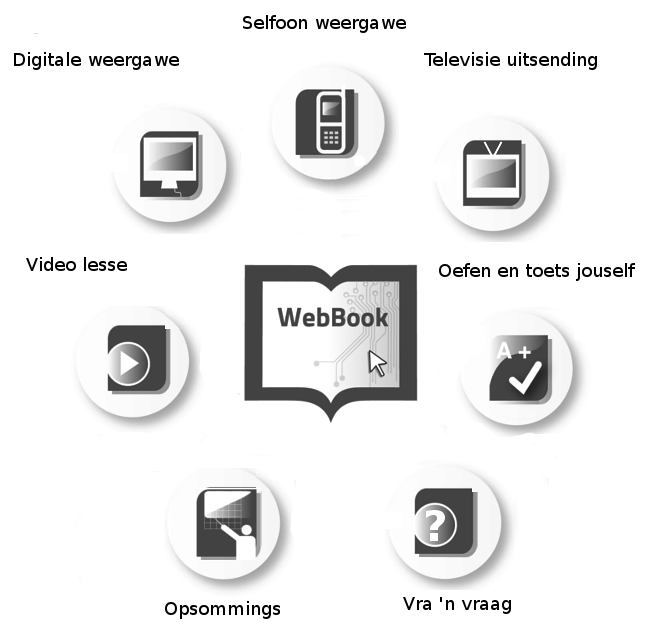
\includegraphics[width=0.70\textwidth]{../title_images/morethantextbookAfrikaans.png}
\end{center}

\par
{\Large
% \textbf{\textit{Everything Maths}} is not just a Maths textbook. It has everything you expect from
% your regular printed school textbook, but comes with a whole lot more. For a start, your learners can download or read it
% online on their mobile phone, computer or iPad, which means you have the convenience of accessing
% it wherever you are.\par
% 
% 
% It is good for learners to hear and read different explanations of concepts as it affords them a more well-rounded understanding of the work. This is why every chapter comes with links to online video
% lessons and explanations, which help bring the ideas and concepts to life. Summary presentations at
% the end of every chapter offer an overview of the content covered, with key points highlighted for easy
% revision.\par
% 
% All the exercises inside the book link to an on-line service where
% learners can get more practice, see the full
% solutions or test their skills level on mobile and PC. Every educator knows that the key to success in maths is practice, practice, practice!
% \par
% 
% 
% We are interested to know what you as an educator think about our books, as well as what the learners
% wonder about or struggle with as they make their way through the content and attempt the exercises. That is
% why we have made it possible for educators and learners to use their mobile phones or computers to access
% the books on-line and digitally pin a question to a page and see what questions and answers other readers
% pinned up too.
% \par

\textbf{Everythings Maths} is nie net ‘n Wiskunde handboek nie. Daar is meer in as net die gewone inhoud wat jy van ‘n skoolhandboek verwag. Om mee te begin kan jou leerders die boek aflaai of aanlyn lees op hul selfoon, rekenaar of iPad. Dit is daarom gerieflik beskikbaar waar ook al jy is.\par

Ons weet dat dit partykeer moeilik is om iets in woorde te verduidelik, daarom is daar lesse en verduidelikings in video-formaat by elke hoofstuk sodat die idees en konsepte vir jou leerders realiteit kan word. Die aanbieding aan die einde van elke hoofstuk bied ‘n oorsig oor al die inhoud wat leerders geleer het, en die kern konsepte is vir hulle uitgelig sodat hulle die maklik kan hersien. \par

Al die oefeninge in die boek het ‘n skakel na ‘n diens wat vir leerders nog oefeninge gee, die oplossings gee of hulle toelaat om hulle vaardigheid te toets – op ‘n selfoon of ‘n rekenaar. \par

Ons wil weet wat jy - die opvoerder - dink, en waaroor jou leerders wonder, waarmee hulle sukkel terwyl hulle deur die boek werk en die oefeninge probeer doen. Ons het dit daarom moontlik gemaak dat opvoerders en leerders hulle werk, met 'n selfoon of rekenaar, digitaal kan “aansteek” op ‘n bladsy en dan ook te kan sien watter vrae en antwoorde ander lesers “aangesteek” het. \par



% This book is the same one used by Mindset Learn in their new television broadcast, where experienced educators work through it, explain the concepts and work out exercises from the book.
}




% mobile or PC
\newpage
\thispagestyle{empty}

{\normalfont\sffamily\fontsize{22}\normalfont\itshape Lees dit op jou selfoon of rekenaar} \par

{\Large
% Learners can have this textbook at hand wherever they are – whether at home, on the the train or at school.
% They can browse the on-line version of Everything Science on their mobile phone, tablet or computer. To
% read it off-line, a PDF or e-book version can be downloaded. Learners can also access Everything Maths
% and Everything Science for not only Grade 10, but also for Grades 11 and 12 on their mobile phone! There is
% now no excuse for a learner to not have these textbooks in front of them in class!

% To read or download the textbook on their phone or computer, direct learners to

Leerders het altyd toegang tot die handboek, of hulle by die huis, die skool of op ‘n trein is. Hulle kan deur na die aanlyn weergawe van Everything Maths op hul selfoon, “tablet” of rekenaar blaai. As hulle dit wil lees terwyl hul van lyn af is, kan hulle dit as ‘n PDF-leêr of in e-boek formaat aflaai. Leerders kan ook toegang Everything Maths en Everything Science vir nie net Graad 10 nie, maar ook vir Graad 11 en 12 op hulle selfoon! Daar is nou geen verskoning vir 'n leerder nie hierdie handboeke in die voorkant van hulle in die klas!\par

Om die handboek op 'n selfoon of rekenaar te lees, verwys leerders na: 

 \\ \underline{www.everythingmaths.co.za}} \vspace*{2cm}






\begin{center}
\begin{minipage}{0.4\textwidth}
\centering
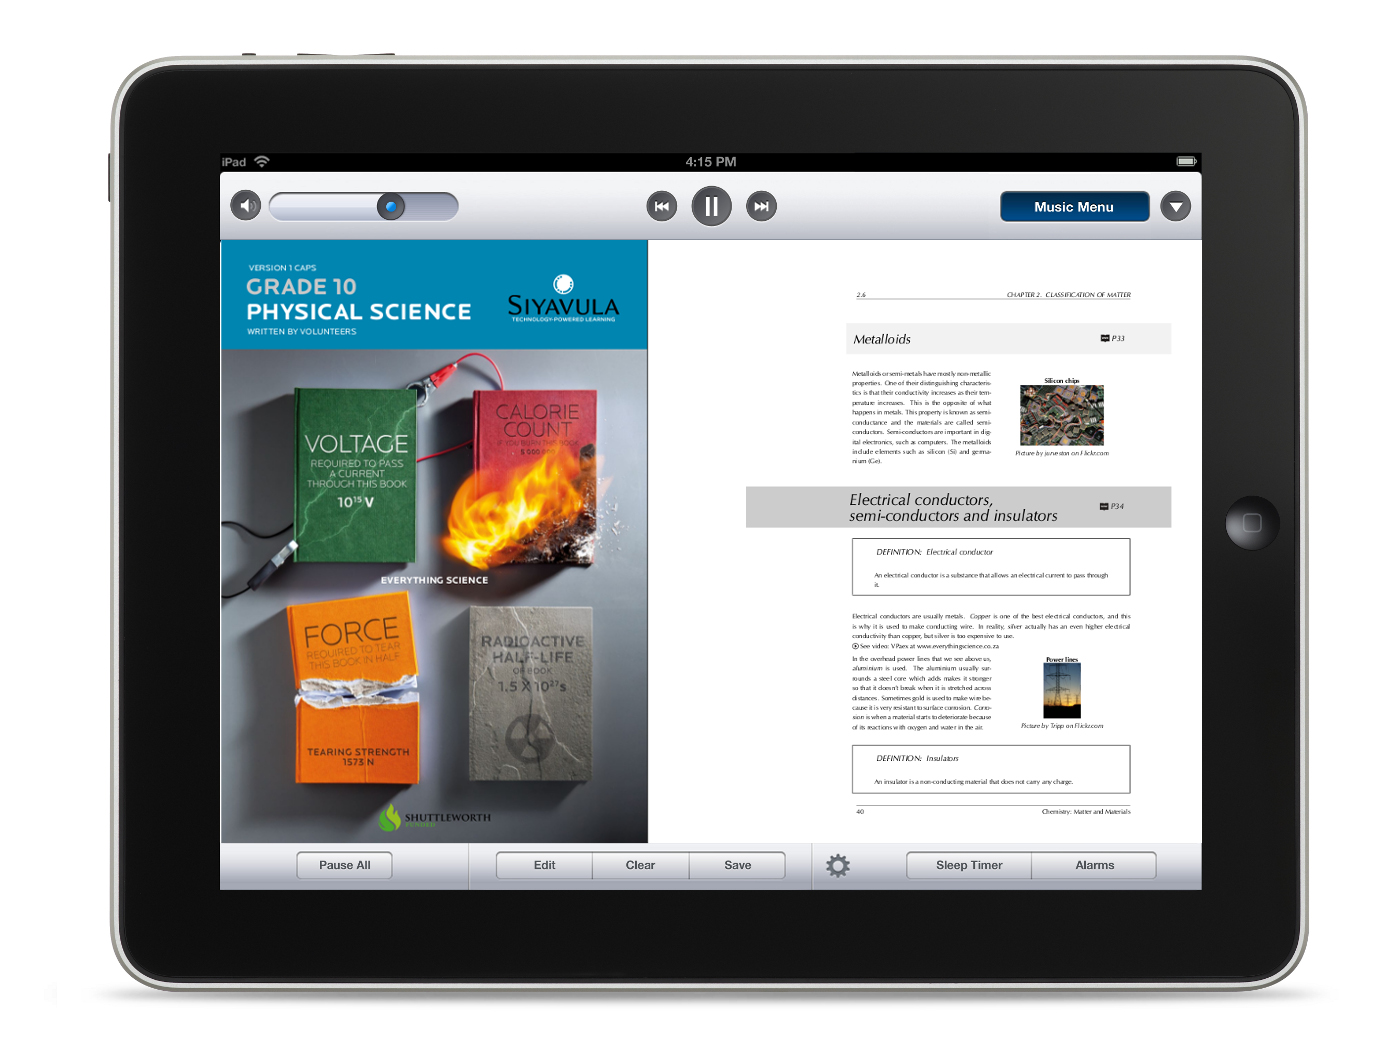
\includegraphics[width=1\textwidth]{../title_images/ipad.jpg}
\end{minipage}
\begin{minipage}{0.4\textwidth}
\centering
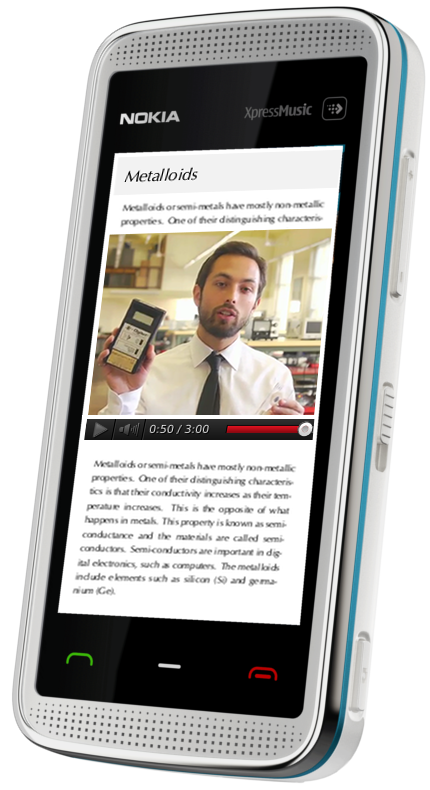
\includegraphics[width=0.4\textwidth]{../title_images/phone.png}
\end{minipage}
\end{center}

\vspace*{2cm}


{\normalfont\sffamily\fontsize{22}\normalfont\itshape Gebruik die ikons en kortkodes} \par

{\Large
% Inside the book you will find these icons to help you and your learners spot where online videos, presentations, practice tools
% and more help exist. The short-codes next to the icons allow you to navigate directly to the resources
% on-line without having to search for them. Visit \underline{www.everythingmaths.co.za} and enter the short-codes in the navigation box.\par

Die ikons in die boek help jou en jou leerders om te sien waar videos, aanbiedinge, oefeninge en ander hulp voorkom. Die kortkodes langs die ikons laat jou toe om direk na die aanlyn-bron te blaai sonder om daarvoor te soek. Gaan na die Everything Maths webblad by \underline{www.everythingsmaths.co.za} en voer die kortkode in die soek-blokkie in.\par

\begin{tabular}{lcl}
\raisebox{-0.8em}{
\includegraphics[width=0.8cm]{../../icons/www.pdf}} & (A123) & Gaan direk na 'n afdeling\\
\raisebox{-0.8em}{
\includegraphics[width=0.8cm]{../../icons/video.pdf}} & (V123) & Video, simulasie of aanbieding \\
\raisebox{-0.8em}{
\includegraphics[width=0.8cm]{../../icons/aplus.pdf}} & (P123) & Oefen en toets jou vaardighede \\
\raisebox{-0.8em}{
\includegraphics[width=0.8cm]{../../icons/help.pdf}} & (Q123) & Vra vir hulp of vind 'n antwoord \\
\end{tabular}
\par
\vspace*{1cm}

% To watch the videos on-line, practise your skills or post a question, go to the \textit{Everything Maths} website at \underline{www.everythingmaths.co.za} on your mobile or PC and enter the short-code in the navigation box.
}




% video lessons
\newpage
\thispagestyle{empty}

{\normalfont\sffamily\fontsize{22}\normalfont\itshape Video-lesse} \par

{\Large
% 
% Look out for the video icons inside the book. These will take you to online video lessons created by Mindset
% Learn and the Khan Academy that help bring the ideas and concepts on the page to life. Learners can now get extra insight, detailed
% explanations and worked examples, while also seeing the concepts in action and hearing real people talk about how they use maths and science in their work!  \par
% 
% This is a great way for you to bring technology into your classroom – using a projector or digital whiteboard, access the books on \underline{www.everythingmaths.co.za} and use the videos to provide an additional summary of the concepts you have covered by offering an alternative explanation. After hours, learners that need additional help will know that they can watch the videos in their own time, with the added bonus of being able to stop, pause and rewind the explanation until they have fully grasped the concept. This is great for revision purposes too, as it is like having a personal teacher on hand for every learner, at any time! \par
Soek die video ikons in die boek. Hierdie ikons neem jou na video-lesse wat sal help om die idees en konsepte vir jou lewendig te maak. Leerders kan ekstra insigte, volledige verduidelikings en uitgewerkte voorbeelde hier sien. Die konsep word prakties voorgestel en jy kan luister hoe regte mense wiskunde en wetenskap in hul werk gebruik. \par

Dit is 'n goeie manier vir jou tegnologie in jou klaskamer te bring - die video's kan' n bykomende opsomming van die begrippe wat jy gedek het deur die aanbied van 'n alternatiewe verduideliking. Na-ure, sal leerders wat addisionele hulp moet weet dat hulle die video's kan sien in hulle eie tyd, met die bonus in staat is om te stop, breek en die verduideliking rewind totdat hulle die konsep ten volle begryp. Dit is ook ideaal vir hersiening, want dit is soos 'n persoonlike onderwyser aan die hand vir elke leerder, te eniger tyd!\par

\begin{figure}[h]
\begin{center}
Sien video verduideliking \raisebox{-0.6em}{
\includegraphics[width=0.7cm]{../../icons/video.pdf}} (Video: V123)\\
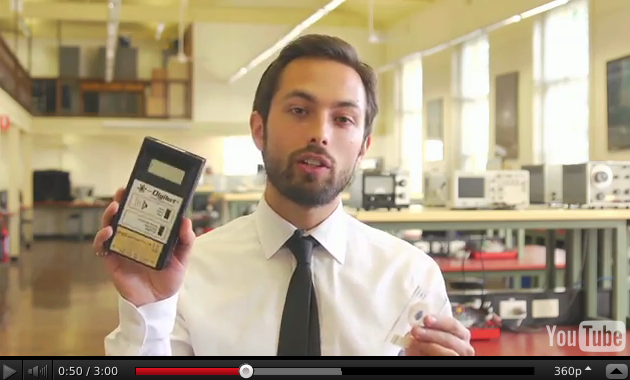
\includegraphics[width=0.5\textwidth]{../title_images/veritasiumvideo.png}
\end{center}
\end{figure}

}


\vspace{0.5cm}
{\normalfont\sffamily\fontsize{22}\normalfont\itshape Video oefeninge} \par

{\Large
As daar oefeninge in die boek is, sal jy die ikons en kortkodes vir video-oplossings, oefeninge en hulp sien. 

%  By entering these short-codes into the box on our website, learners will be taken to video solutions of select exercises to show them
% step-by-step how to solve such problems. Encourage your learners to access these video exercises, which are great for revision purposes as well as to reinforce your own teaching.\par
Hierdie short-codes vat jou na die video-oplossings van sommige oefeninge sodat jy stap-vir-stap kan sien hoe om die probleem op te los. Moedig jou leerders om hierdie video oefeninge, wat 'n groot vir hersiening, sowel as om toegang te verkry tot jou eie onderrig te versterk.

Jy kan toegang tot die videos kry deur:
\begin{itemize}[noitemsep]
\item hulle aanlyn op jou selfoon of rekenaar te kyk
\item die videos af te laai sodat jy die van lyn af op jou selfoon of rekenaar kan kyk.
\item ‘n DVD te bestel wat jy op jou TV of rekenaar kan speel.
\item dit van lyn af af te laai met Bluetooth of Wi-Fi van sekere afsetpunte
\end{itemize}
% For additional viewing, downloads or more information, visit the \textit{Everything Maths} website on your phone or computer at \underline{www.everythingmaths.co.za}.
\begin{figure}[H]
\begin{center}
Sien video oefening \raisebox{-0.6em}{
\includegraphics[width=0.7cm]{../../icons/video.pdf}} (Video: V123)\\ 
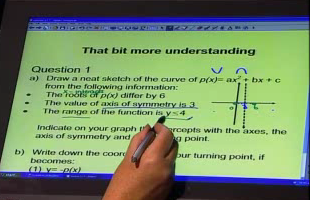
\includegraphics[width=0.5\textwidth]{../title_images/mindsetexercise.png}
\end{center}
\end{figure}
\\
Om nog videos te sien, of vir meer inligting, besoek die Everything Maths webblad vanaf jou selfoon of rekenaar by \underline{www.everythingmaths.co.za}    \par


\vspace*{1cm}
}


% monassis
% \newpage
% \thispagestyle{empty}

{\normalfont\sffamily\fontsize{22}\normalfont\itshape Stel toetse met Monassis op} \par

{\Large
Siyavula bied 'n oop aanlyn assesseringsbank, genoem Monassis, aan, vir die deel en toegang tot  kurrikulum belynde toets- en eksamenvrae met antwoorde. Al die vrae en oplossings wat in die handboek gevind word, is beskikbaar op Monassis. Daarbenewens stel hierdie webwerf opvoeders in staat om vinnig toetse en vraestelle op te stel deur items van die databasis te kies en dit by hul toetse te voeg. Opvoeders kan dan die toets en memorandum, wat gereed is om gedruk te word, afsonderlik aflaai. Monassis bied ook die opsie aan opvoeders om hul leerders se punte in te voer om 'n verskeidenheid diagnostiese verslae oor die leerders se vordering terug te kry.\par


\begin{figure}[h]
\begin{center}
\raisebox{-0.6em}{

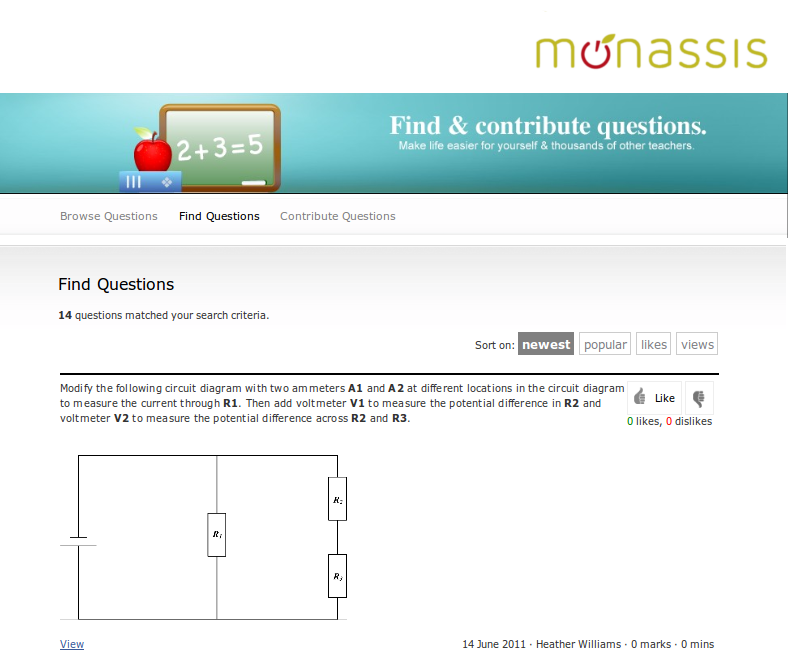
\includegraphics[width=0.5\textwidth]{../title_images/monassis.png}}
\end{center}
\end{figure}


%ENGLISH HERE
Ons moedig jou aan om gebruik te maak van die eenvoudige funksionaliteit wat jou help deur tyd te spaar met die opstel van toetse en die analise van leerders se punte. Vir meer inligting besoek \underline{www.monassis.com}.\par






% {\normalfont\sffamily\fontsize{16}\normalfont\itshape  How do I do Each of These?}\par 
% \textbf{Share and access questions}\par 
% Sharing questions: use either the online editor or OpenOffice template which can be downloaded from the website (Browse questions → Contribute questions → Import questions). Take your test/worksheet/other question source. Break it up into the smallest sized individual questions that make sense, and use the template style guide to style your page according to question/answer. Upload these questions or type them up in the online editor (Browse questions → Contribute questions → Add questions). Do not include overall question numbering but do include sub numbering if needed (e.g. 1a, 2c, etc.). Insert the mark and time allocation, tag questions according to grade, subject i.e. a description of the question, and then select the topics from the topic tree. Finalise questions so that they can be used in tests and accessed by other Monassis users.\par 
% 
% Accessing questions: there are three ways to access questions in the database. Click on “Browse questions” → click on the arrow to the left of the grade, which opens out the subjects → keep clicking on the arrows to open the learning outcomes or, following the same process, instead of clicking on the arrow, click on the grade → now you can browse the full database of questions for all the subjects in that grade or, from the landing page, click on “Browse questions” → below the banner image click on “Find Questions” → search by topics, author (if you know a contributor), text or keywords e.g. Gr10 mathematics functions and graphs. \par 
% 
% \textbf{Create tests from questions
% }\par 
% So, you have all these bits of tests (i.e. many questions!), but what you really want is the actual test. How do you do this? Well, you can simply click “add to test” on any question and then click on the “Tests” tab at the top right of the page, and follow the simple instructions. Alternatively you can create a test by starting with clicking on that same “Tests” tab, and add questions to your test that way. Once done, simply print off the PDF or Word file of the questions, issue your test, collect them once complete, and mark them using the memo provided by Monassis. \par 
% 
% \textbf{Create class lists}\par 
% 
% But now you are asking, how can I keep track of my classes? Is Johnny Brown in class A or B? Well, you can make a class list by clicking on the “Class lists” tab at the top right of the page, and either import a CSV file, or manually enter the relevant information for each class. Now you can issue tests  to your classes, and have a class list for each class. And what about capturing their marks?\par 
% 
% \textbf{Create scoresheets}\par 
% For each test you can create a scoresheet. Select the “Tests” tab at the top right, click on “Marks” below the banner image, and select the test and follow the instructions to input their marks. You can then export these as a CSV file for use in spreadsheets.\par 
% 
% \textbf{Analyse learners' performance}\par 
% 
% And finally, you can print out reports of class performance. Click on “Reports” at the top right of the page, which opens various reports you can view. There are reports to see class performance, learner performance, class performance per topic, class performance per question, learner strengths and weaknesses, and learner progress.\par 
% So now you know how Monassis works, we encourage you to make use of its simple functionality, and let it help you save time setting tests and analysing learner marks!\par 
% 
}





% practise and test your skills
\newpage
\thispagestyle{empty}
{\Large


{\normalfont\sffamily\fontsize{22}\normalfont\itshape Intelligente oefening vir leerders} \par

% One of the best ways for learners to prepare for tests and exams is to practice answering the same kind of questions they will be tested on. At every set of exercises you will see a practice icon and short-code, which link to an online database for learners to practice further exercises. Point your learners at \underline{www.everythingmaths.co.za} on their mobile phone or PC. where they can enter the short-code from the textbook into the box on the website, and be redirected to additional exercises online. This on-line practice on mobile and PC will keep track of learners' performance and progress, give them feedback on areas which require more attention, and suggest which sections or videos to look at.\par

Een van die beste maniere om vir die leerders voor te berei vir toetse en eksamens is om te oefen om dieselfde soort vrae wat hulle sal getoets word te beantwoord. By elke stel oefeninge sal jy sien 'n oefening ikoon en kort-kode.
Vir leerders om te oefen en om hul vaardighede te toets, verwys hulle na \underline{www.everythingmaths.co.za} op hulle selfoon of rekenaar, en voer die kort-kode in die boks.
Hierdie aanlyn oefening op selfoon of rekenaar sal boekhou van leerders se prestasies en vordering, vir hulle terugvoer gee oor areas wat meer aandag benodig en voorstelle maak oor seksies en videos om na te kyk. \par


\begin{figure}[H]
\begin{center}
Sien meer oefening \raisebox{-0.6em}{
\includegraphics[width=0.7cm]{../../icons/aplus.pdf}} (QM123)\\ 
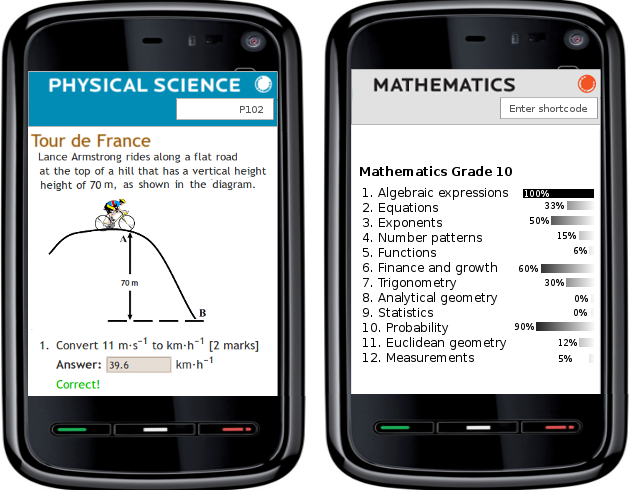
\includegraphics[width=0.65\textwidth]{../title_images/practicephones.png}
\end{center}
\end{figure}
\par
% The software can generate any number of questions with the same structure but different details i.e. the numerical values in physics or maths problems can change each time, but the type of question can stay the same. This allows much more variety than a traditional question bank - to the extent that a different practice test can be created automatically for each student in a class. The system also generates a memorandum along with each test, and tracks the learners' conceptual understanding through their success at answering different types of questions.
Die sagteware kan enige aantal vrae met dieselfde struktuur, maar verskillende besonderhede, genereer b.v. die numeriese waardes in fisika of wiskunde probleme kan elke keer verander, maar die soort vraag kan dieselfde bly. Dit laat baie meer verskeidenheid as 'n tradisionele vraag bank toe, tot die mate dat verskillende oefentoetse outomaties geskep kan word vir elke student in die klas. Die stelsel genereer ook 'n memorandum saam met elke toets, en volg die leerders se konseptuele begrip deur middel van hul sukses om verskillende tipes vrae te beantwoord. 
\par

% This tool aims to discover the strong and weak points in learners' understanding as the learners are going through worked examples and drilling exam problems. By knowing with which concepts learners are struggling, the system can then do useful things like
Hierdie hulpmiddel het ten doel om die sterk- en swakpunte te ontdek in die leerders se begrip soos die leerders vorder, deur middel van uitgewerkte voorbeelde en eksamen probleme. Deur te weet watter begrippe leerders mee sukkel, kan die stelsel nuttige dinge doen soos 
\begin{itemize}[noitemsep]
\item meer oefening voorsien oor die tipe vrae waarmee die leerder sukkel;
\item hersieningsmateriaal  aanbeveel uit vrylik beskikbare opvoedkundige hulpbronne (byvoorbeeld, Siyavula se Everything Maths en Everything Science handboeke);
\item terugvoering vir leerders, opvoeders en ouers gee; verslae oor leerders se vordering en oor die spesifieke konsepte waarvoor hulle meer aandag moet gee. 
\end{itemize}
%  The above is done for each learner individually, delivering a customised practice and revision schedule to match his or her pace and understanding.
Die bogenoemde word gedoen elke leerder op 'n individuele basis, die lewering van 'n persoonlike oefening- en hersieningsskedule wat by sy of haar pas en begrip pas. \par



% For learners to practice and test their skills, point them at \underline{www.everythingmaths.co.za} on their mobile phone or PC and enter the short-code in the box.\par

\vspace*{1cm}
}
\\
{\normalfont\sffamily\fontsize{22}\normalfont\itshape Help leerders om antwoorde te vind} \par

{\Large
%ENGLISH
Ons verstaan dat onderwysers nie altyd beskikbaar is wanneer 'n leerder 'n vraag het nie, veral na-ure. Jou leerders kan nou die handboek op hul selfoon of rekenaar oopmaak.

Leerders moet die kort-kodes op artikel opskrifte gebruik om na die plek in die boek, en die kort-kodes vir die oefeninge vir die hulp met spesifieke vrae.\par




\begin{tabular}{lcl}
\raisebox{-0.8em}{
\includegraphics[width=0.8cm]{../../icons/www.pdf}} & (P78) & Besoek hierdie afdeling om vrae te kyk of te pos \\

\raisebox{-0.8em}{
\includegraphics[width=0.8cm]{../../icons/help.pdf}} & (QM123) & Vra vir hulp of vind 'n antwoord\\
\end{tabular}
\par
\vspace*{1cm}

\begin{figure}[H]
\centering
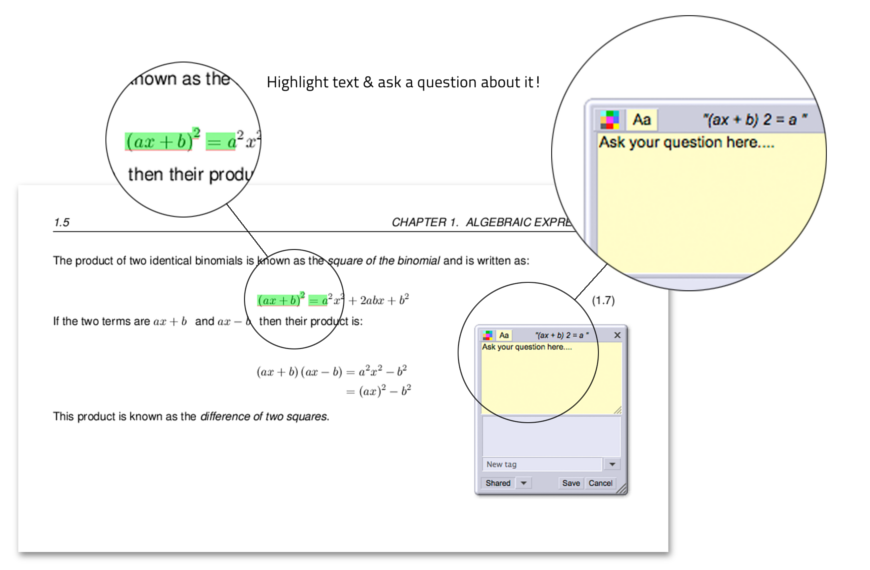
\includegraphics[width=\textwidth]{../title_images/questions.png}
\end{figure}

% Using the short-codes at section headings and exercises in the textbook, learners can go to the above website, enter the short-code into the box on-line, and be redirected to the relevant place in the book. Once there they can pin their question at the exact spot where it cropped up (see image below), by highlighting a specific section of the text. They will be able to see whether the question has been asked before by other learners, and what the given answer to that question is. \par
% Look out for these icons in the texbook: \par
% Visit the Everything Maths website on your phone or computer at \underline{www.everythingmaths.co.za }\par
}
\pagebreak
{\normalfont\sffamily\fontsize{22}\normalfont\itshape Vertel ons hoe om die boek te verbeter } \par

{\Large
As jy enige kommentaar, gedagtes of voorstelle op die boeke, besoek \underline{www.everythingmaths.co.za}, oorskakel na die opvoeder af, en die gebruik van ons annoteerder instrument, kan jy vang dit in die teks. Dit kan wissel van wenke en idees te deel met jou mede-opvoeders, om te bespreek hoe om beter konsepte in die klas verduidelik. Ook, as jy enige foute in die boek opgetel het, kan jy 'n kennis van hulle hier maak, en sal ons hulle in die tyd vir die volgende oplaag korrekte.
 \par


\begin{figure}[H]
\centering
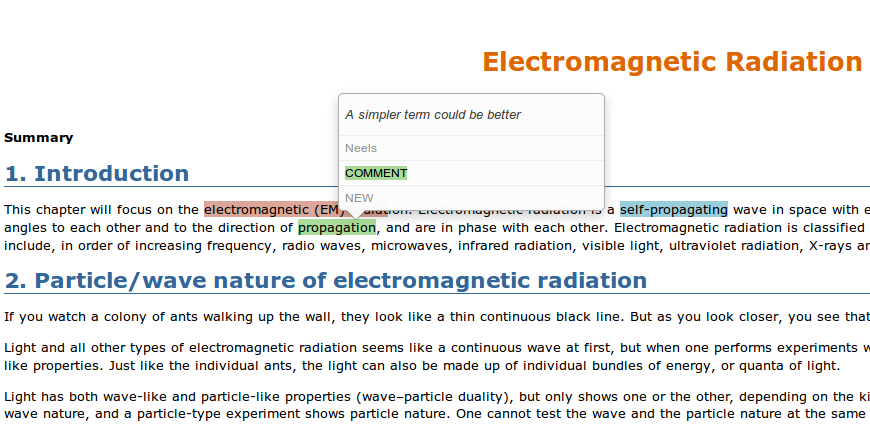
\includegraphics[width=\textwidth]{../title_images/annotater.png}
\end{figure}


% Look out for these icons in the texbook: \par
% Visit the Everything Maths website on your phone or computer at \underline{www.everythingmaths.co.za }\par
}
% %television
% \newpage
% \thispagestyle{empty}
% {\normalfont\sffamily\fontsize{22}\normalfont\itshape Television broadcasts} \par
% This book is the same one used by \textbf{Mindset Learn} in their television broadcast where experienced
% educators explain the key concepts, perform live experiments and work out exercises from the book.
% \textbf{Mindset Learn} broadcasts a full 28 hours of curriculum support each week of term. \par
% 
% 
% Maths can be seen on Mondays and Science on Tuesdays. There is also Life Sciences on Wednesdays
% and Maths Literacy on Thursdays. Revision of the week's work is done on Saturdays for Grade 12 and on
% Sundays for Grades 10 and 11.
% 
% 
% }
%ask questions, find answers
% \newpage
% \thispagestyle{empty}


% 
% 
% 
% 
% {\Large
% 
% \begin{table*}[h]
% \large
% \begin{tabular}{lll}
% \textbf{Maths and Science Broadcasts}&&\\
% Grade 10  Maths & Mondays at 4pm & Every second Sunday at 1pm\\
% Grade 11  Maths & Mondays at 5pm & Every second Sunday at 9am\\
% Grade 12  Maths & Mondays at 6pm & Every Saturday at 9am\\
% Grade 10  Science & Tuesdays at 4pm & Every second Sunday at 1pm\\
% Grade 11  Science & Tuesdays at 5pm & Every second Sunday at 9am\\
% Grade 12  Science & Tuesdays at 6pm & Every Saturday at 11am\\
% \textbf{Other broadcasts} & & \\
% Grade 10  Life Science & Wednesdays at 4pm & Every second Sunday at 3pm\\
% Grade 11  Life Science & Wednesdays at 5pm & Every second Sunday at 9am\\
% Grade 12  Life Science & Wednesdays at 6pm & Every Saturday at 1pm\\
% Grade 10  Maths Literacy & Thursdays at 4pm & Every second Sunday at 3pm\\
% Grade 11  Maths Literacy & Thursdays at 5pm & Every second Sunday at 9am\\
% Grade 12  Maths Literacy & Thursdays at 6pm & Every Saturday at 3pm\\
% \end{tabular}
% \end{table*}
% 
% \\
% \textbf{You can watch these live sessions on:}
% \begin{itemize}
%     \item Mindset free-to-air for schools (ask your school)
%     \item Channel 319 on DStv
%     \item TopTV on 319 
% \end{itemize}
% 
% 
% }








% Put the margins back for the rest of the book

\newgeometry{lmargin=0.1\paperwidth, rmargin=0.25\paperwidth, tmargin=1in, bmargin=1in, twoside, centering, includehead,  marginparwidth=0.225\paperwidth}

\normalfont
